% !TEX root = ../../../main.tex
% 来源：中学数学实验教材·第三册（高中数学）
% 章节：三角函数的图象和性质 / 正弦型曲线
% 原始文件：7.tex，行 1289-1314
% 类型：tikz
% ---
\begin{tikzpicture}[>=latex]
\draw [->](-1,0)--(7.8,0)node[right]{$x$};
\draw [->](0,-3)--(0,3)node[right]{$y$};
\foreach \x in {-1,-2,1,2}
{
    \draw(0,\x)node[left]{$\x$}--(.1,\x);
}

\node at (-.2,-.2){$O$};

\foreach \y in {1,2,.5}
{
    \draw [domain=0:7, samples=1000, thick] plot(\x, {\y*sin(\x r)});
}

\draw (.5*pi,0)node[below]{$\frac{\pi}{2}$}--(.5*pi,.1);

\draw (1.5*pi,0)--(1.5*pi,.1)node[above]{$\frac{3\pi}{2}$};

\node at (pi-.2,0)[below]{$\pi$};
\node at (2*pi+.2,0)[below]{$2\pi$};

\node at (7,.3)[right]{$y=\tfrac{1}{2}\sin x$};
\node at (7,.9)[right]{$y=\sin x$};
\node at (7,1.5)[right]{$y=2\sin x$};
\end{tikzpicture}
